\documentclass[10pt]{article}
\usepackage{graphicx,amssymb, amstext, amsmath, epstopdf, booktabs, 
verbatim, gensymb, geometry, appendix, natbib, lmodern, hyperref, float, titlesec, subfigure}
\geometry{letterpaper}
%\usepackage{garamond}

\newcommand*\Title{Neurowrx Account Manual}
\newcommand*\cpiType{some subtitle}
\newcommand*\Date{Novermber 2018}
\newcommand*\Author{Michael Braeutigam}
\title{Neurowrx Account Manual}
\author{Michael Braeutigam}
\date{\today}
%-----------------------------------------------------------

\usepackage{cpistuff/cpi} % This is what makes your document look like a cpi document.


\begin{document}

\begin{titlepage}
\maketitle
\end{titlepage}

\linespread{1.15} %Set standard document linespacing

\begin{executive}

This is a document describing the fuctionality of the neurowrx website.

\frame{
\textbf{Important Title}

This is a convenient place to put any necessary legal mumbo-jumbo}
\end{executive}

\tableofcontents









%\subsection{green writing}

%Use the \texttt{callout} command:

%\callout{By the shores of gitchee gumee\\ by the shining big sea waters \\ stood the wigwam of Nokomis \\ brother of the moon, Nokomis.}



%Use the \texttt{frame} command:

%\frame{ 'Twas brillig and the slithy toves did gyre and gimble in the wabe \\ all mimsy were the borogroves, and the mome raths outgrabe. \\ Beware the Jabberwock, my son, the claws that bite, the jaws that snatch \\ Beware the Jubjub bird, and shun the frumious Bandersnatch.}

%\ref{accountemail} returns the index of the figure in the document


\section{Ordinary Members}

\subsection{Account Creation}

\begin{flushleft}
Once you are a neurowrx member, a username (probably based on your actual name, or organization name) will be chosen by the site admin, and you will receive an email at the address that you provided in your application.  It will have neurowrx in the subject line so check your spam filter if you do not receive it promptly.  It will notify you of your username and give you a link to a page where you can set your password, as well as a link to the regular login panel.  The login panel can be reached though this link or though the main site at \url{https://neurowrx.org/}, by clicking on the button at the top right corner. 
\end{flushleft}

\begin{figure}[h]
\centering
\caption{A typical account creation email}
\label{accountemail}
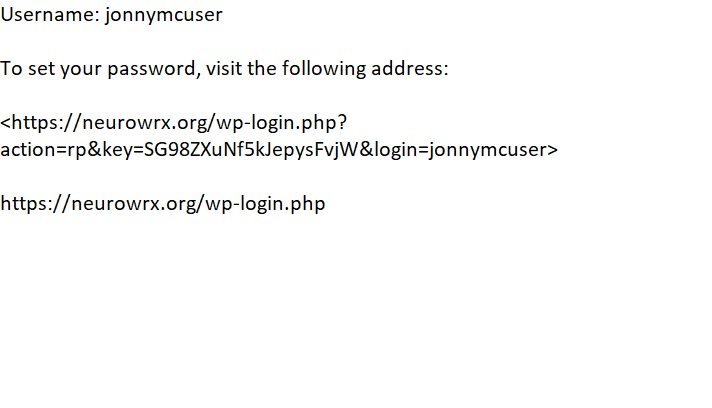
\includegraphics[scale=1.0]{images/accountcreation.jpg}
\end{figure}

The account's password is initially randomized and should be set via the first link before one attempts to log in.  In the case that the password is forgotten, it can be recovered though a link on the main login page at \url{https://neurowrx.org/wp-login.php}.

\begin{figure}[h]
    \centering
    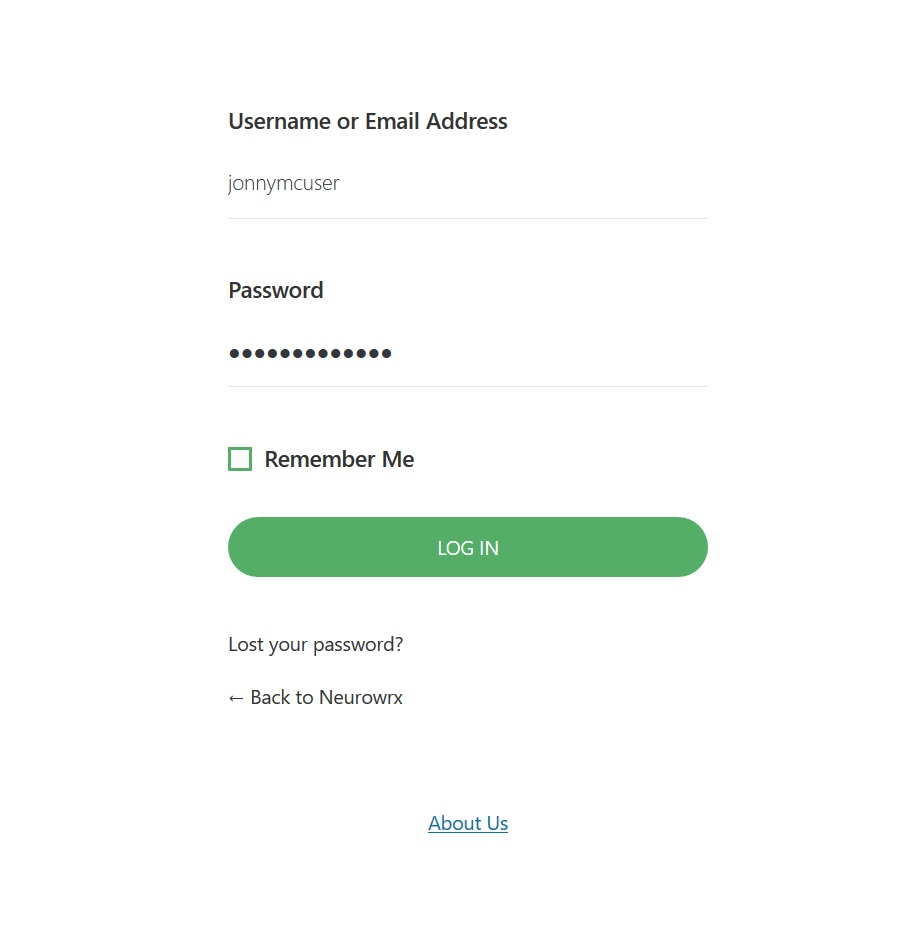
\includegraphics[scale=0.3]{images/loginpage.jpg}
    \caption{The login page}
    \label{loginpage}
\end{figure}

\begin{flushleft}
After you have chosen your password, you can log in with either your username, or with your email address.  Both are required to be unique, and in the case that you have more than one account; you must provide distinct email addresses for distinct accounts. 
\end{flushleft}

\begin{flushleft}
Once a successful login has occurred, the top panel of the website changes to give the user access to the communication features.  A link for the members section appears, as well as an icon for private messages, notifications, and another for settings.  There is also a menu hiding under the profile picture with more features which will be discussed in succeeding sections. 
\end{flushleft}

\begin{figure}[h]
    \centering
    
\includegraphics[scale=0.3]{images/topbar.jpg}
    \caption{The top panel that is publicly visible}
    \label{topbar}
\end{figure}

\begin{figure}[h]
    \centering
    
\includegraphics[scale=0.3]{images/topbarlogged.jpg}
    \caption{The top panel after login}
    \label{topbarlogged}
\end{figure}

\subsection{Your Neurowrx profile}

\begin{flushleft}
By hovering the mouse over the profile pic, a dropdown menu (with association submenus) becomes available.  The profile functions can either be accessed though the profile submenu or by clicking on "profile" itself to go to the profile page.  
\end{flushleft}

\begin{figure}[H]
    \centering
    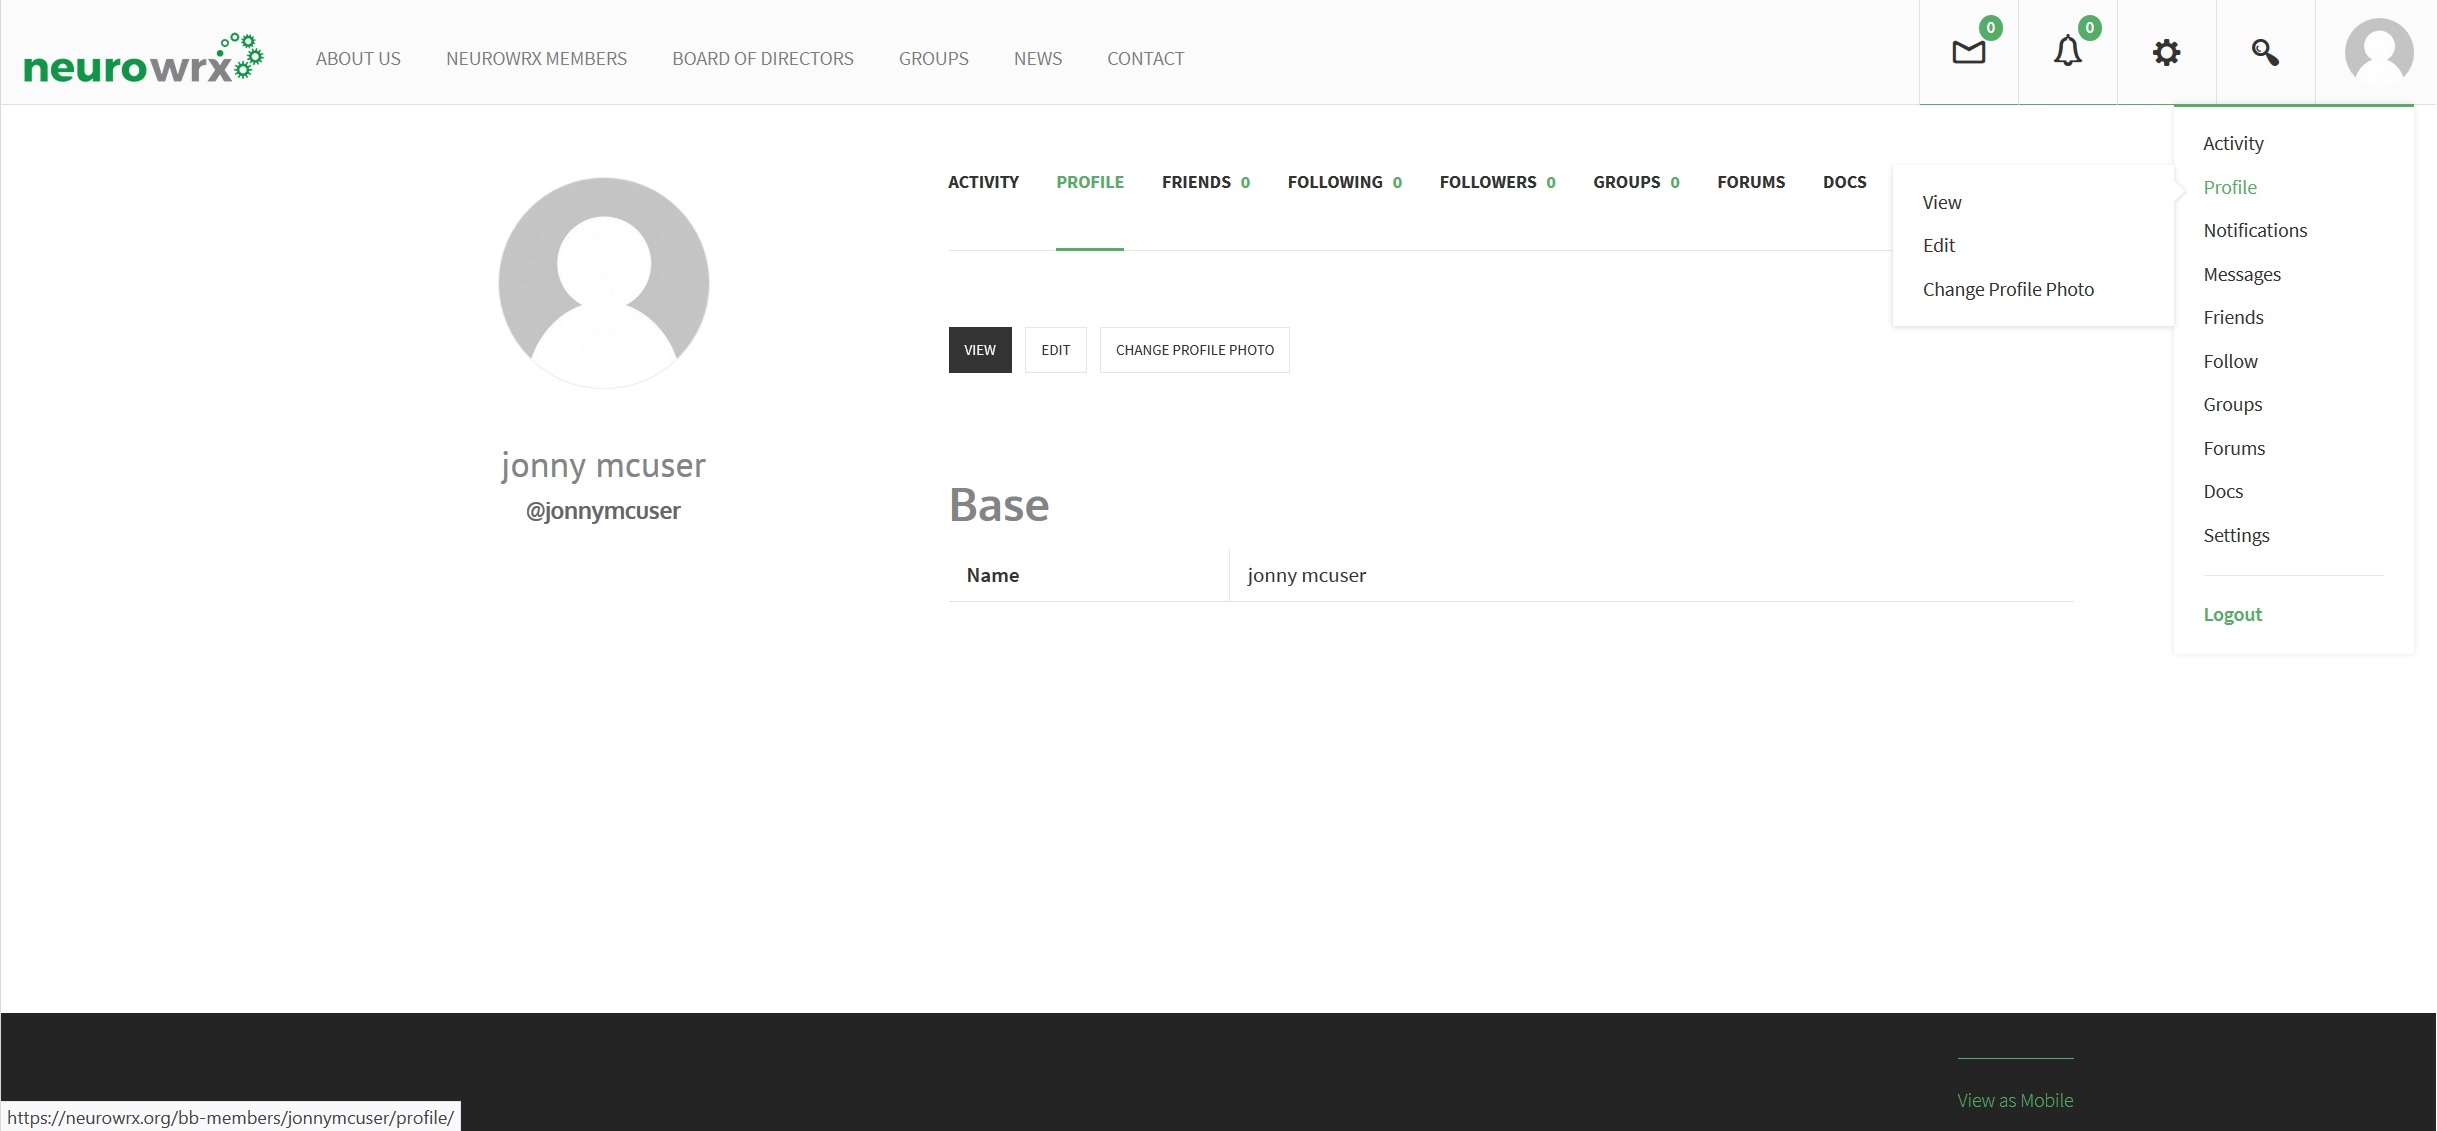
\includegraphics[scale=0.2]{images/profile.jpg}
    \caption{The profile page, and the profile menu that can be used to navigate to it.}
    \label{profilepage}
\end{figure}

\subsubsection{Changing your profile picture}

\begin{flushleft}
When you add a profile picture (which is optional), you can either upload an existing file by dragging the file into the hatched boundary box (which doesn't work on all operating systems), open a file selection window by clicking the green button, or click the "Take Photo" link to activate your webcam (assuming that you have one plugged in).  This step makes the an image file available to the cropping tool, which you will use to select a small square shaped section of the image (presumably your face) for use as your face on the forums and in the messaging system. 

\end{flushleft}
 The image is required to be of the .jpeg, .gif, or .png file formats.  It is also recommended that you use an image that is of at least 280x280 pixels, but this isn't strictly necessary. 
\begin{flushleft}

\end{flushleft}

\begin{figure}[h]
    \centering
    \subfloat{{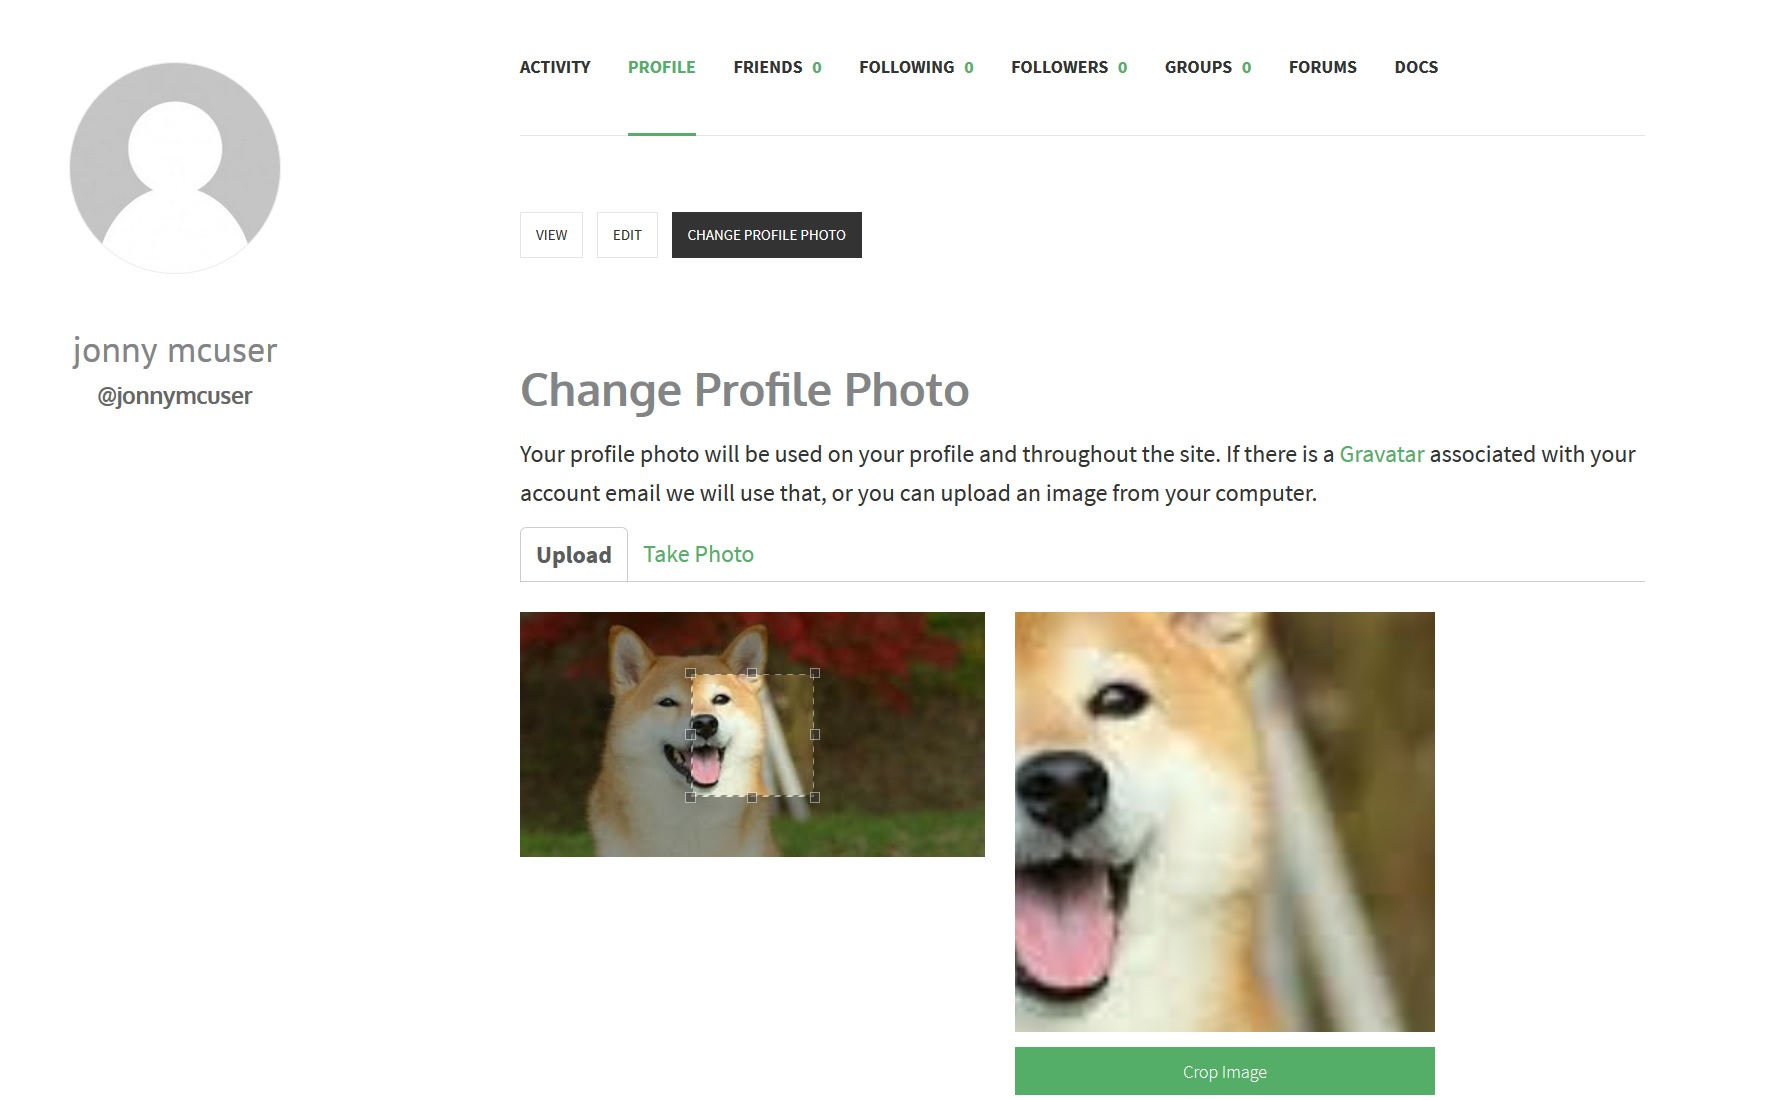
\includegraphics[scale=0.2]{images/doggy.jpg}}}
    \qquad
    \subfloat{{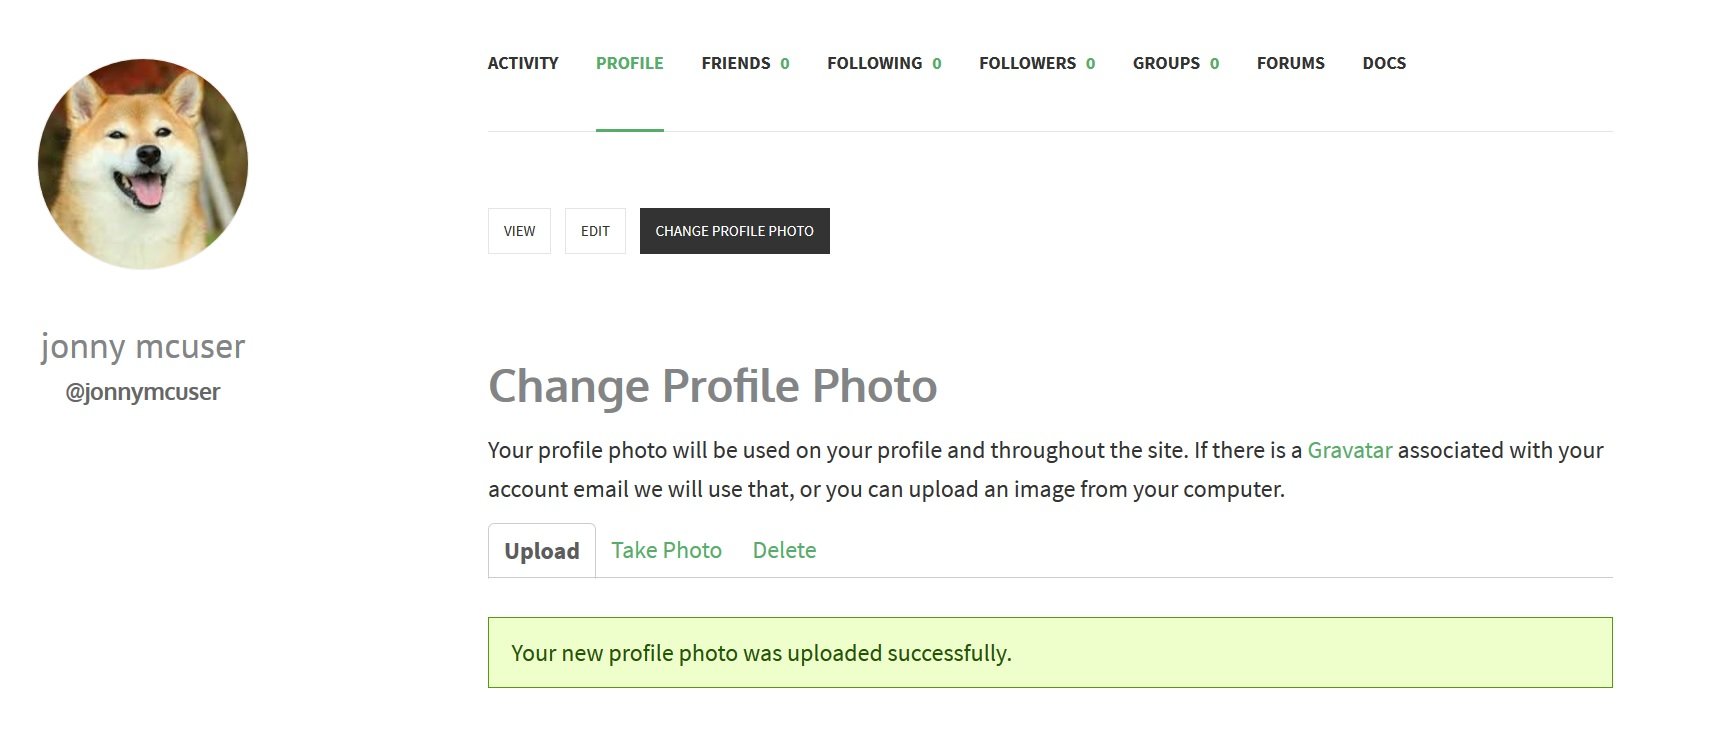
\includegraphics[scale=0.2]{images/doggy2.jpg}}}
    \caption{A successful profile picture upload}
    \label{avatarUp}
\end{figure}

\subsubsection{Editing your other profile information}

\begin{flushleft}
Other than the photo, your Neurowrx profile contains a changeable public Name field (which is not the same as your username) a gender field (which by default has neither selected, and does not have to be chosen) and several fields that you can paste links to your profiles on other social networking services.  At the time of this writing, we have fields for facebook, twitter and a few others.  This list could potentially grow in the future.  
\end{flushleft}

\begin{flushleft}
One is only expected to post the url of the profile in question, the form of which varies from service to service.  If you are unsure what the url to your profile is, consult the documentation for that particular service. 
\end{flushleft}


\subsection{Groups}
\begin{flushleft}

\end{flushleft}

\subsubsection{Joining Groups}
\subsection{Uploading Documents}
\subsection{Messaging}

\section{Group Moderators}
\section{Administrators}


\bibliography{codes_impact}
\bibliographystyle{plainnat}

\end{document}